\chapter{基于异构计算的自适应计算任务分配}

本章首先探讨了移动端SoC的发展趋势及其对深度学习模型于移动端进行离线推断的影响。3.2节通过对比分析CNN前向推断于手机GPU和CPU上的执行能效详细阐述了使用移动设备上所有可获得的本地异构处理器运行CNN模型推断并非是一种高能效的方式。3.3.1节提出了一种无需人为干预、可自适应计算目标移动平台上所有本地处理器能效的算法。使用该算法可进一步获得目标移动平台上可用于执行CNN前向推断的高能效设备处理器组合。3.3.2节给出了一种为所选择设备处理器组合分配计算任务的方法。3.3节基于ODROID-XU3平台实现了本文所提出的算法,并验证了这些算法的有效性。

\section{移动端SoC的发展趋势}
多核异构CPUs(如,ARM的big.LITTLE\cite{chung2012heterogeneous})已然成为当前移动设备处理器的主流架构,而GPUs也已集成到绝大部分的移动设备中。GPUs与生俱来的并行计算能力很适合用来处理深度模型中的常见计算类型。然而,处理能力较强的GPUs也会以惊人的速度消耗着移动设备电池电量。事实上,手机GPUs的设计过程中更加重视的是低功耗而不是高性能,所以当前商业上应用的大多数移动GPUs的计算能力并不是很强大,如Mali™-T628 MP6的频率仅为600MHz、核心数仅为6。因此,单独的GPUs解决方案也不能够满足移动平台上深度学习模型的运行条件。除GPUs外,我们还应该注意到,移动设备中也集成了一些低功耗处理器,如DSPs、LPUs、NPUs等。高通骁龙系列的SoC集成了Hexagon DSP;英伟达的Tegra K1 SoC除了提供了高性能的GPU(192核)、2.3Ghz的4核CPU外,还提供了一个第五代低功耗核LPC;华为的海思麒麟970还内置了神经网络处理单元(NPU),使用NPU可进行高效的 AI相关计算。另外,英伟达如今已跟芯片设计公司ARM达成合作,将开源的NVIDIA深度学习加速器(NVDLA)架构集成到Arm的Project Trillium平台上,从而更好地实现移动端机器学习。在2018年的世界移动通信大会(MWC)上,联发科也宣布推出Helio P60芯片,该芯片使用的ARM Cortex™-A73大核心是专为手机端AI应用设计的处理器架构,可用于实现深度学习面部检测、物体与场景辨识等功能。可以看出,移动端SoC芯片将会越来越多地配备不同用途的专用处理器,并且每一种处理器都拥有着不同的资源特征。

根据层的类型和其他方面的模型特征,使用不同的处理器组合执行不同深度学习模型,这样便可以带来不同的性能-功耗折中。因此,如何高效地利用手机本地各种异构处理器将是移除深度学习模型被嵌入式平台所广泛采用之屏障的关键\cite{attia2015dynamic}。

\section{基于异构计算的CNN推断研究动机}

之前的研究工作要么在CNN推断中没有很好地利用手机移动设备的异构计算能力(如仅使用CPU或GPU进行前向推断),要么总是试图利用所有可获得的本地设备进行模型推断,而本章主要探索如何高能效地使用手机移动设备的异构计算能力完成CNN模型的离线推断过程。

\begin{figure}[htbp]
    \centering
    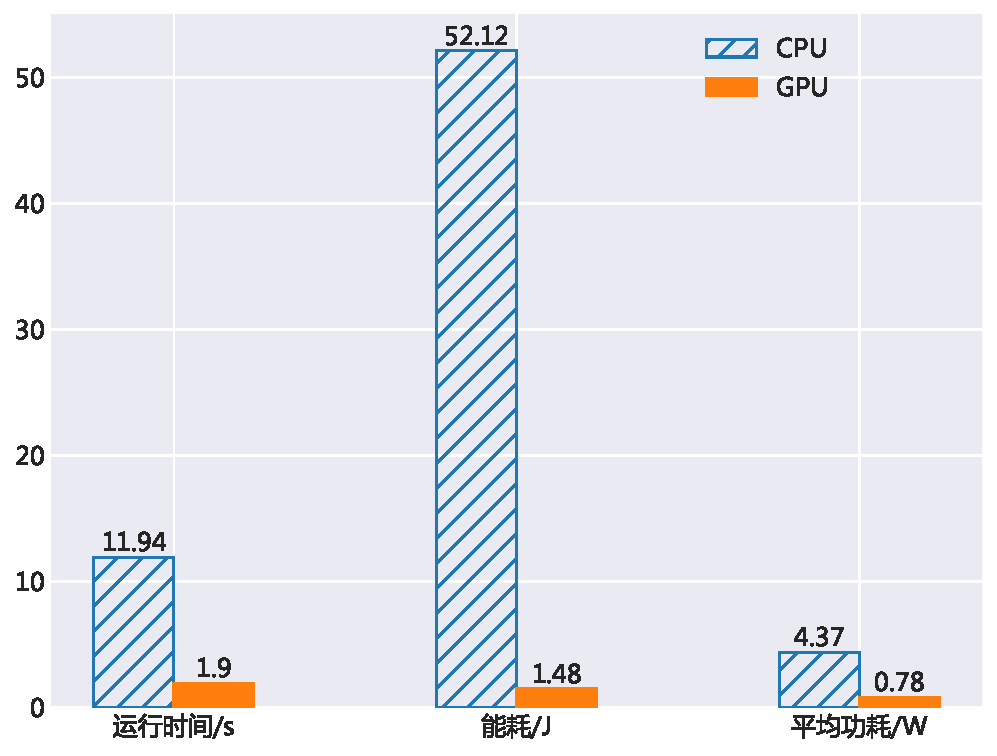
\includegraphics[height=0.4\textwidth]{figures/yolo_energy.pdf}
    \caption{分别于手机GPU和CPU上执行一次完整CNN推断的运行时间、能耗和功耗}\label{figure:figure28}
\end{figure}

图\ref{figure:figure28}显示了分别于手机GPU和CPU上运行一次完整CNN推断所需时间、能耗和功耗。为了充分利用手机CPU的计算性能,在CPU上执行CNN前向推断时使用了ARM处理器提供的NEON指令(一种单指令多数据流)并且启用了与处理器核心数相同的线程。由图\ref{figure:figure28}可知,即使利用了CPU所有的并行处理能力,CPU执行一次完整的CNN前向推断过程仍需要耗时11.94秒、耗能52.12焦。然而,当使用GPU去处理相同的一次推断时,平均运行时间和能耗仅为1.9秒和1.48焦。由此可见,若同时使用手机GPU和CPU并行地执行CNN的前向推断过程,其执行时间肯定会有所降低,但是其能效可能就会很低。原因可以由表\ref{table:table9}所示的EDP能效值得出,其中GPU的推断能效是CPU的221倍。因为手机的电池电量总是有限的,所以手机系统必须为计算过程维持一个较好的执行速度与能耗开销的折中。

\begin{table}[htbp]
  \centering
  \caption{分别于手机GPU和CPU上执行一次完整CNN推断的能效}
  \label{table:table9}
  \begin{tabular}{cc}
    \toprule
      运行处理器 & EDP(Joules*seconds) \\
    \midrule
      CPU & 622.31 \\
      GPU & 2.81 \\
    \bottomrule
  \end{tabular}
\end{table}

基于上述分析,本文得出结论:手机移动平台需要使用一个高能效的本地异构设备处理器组合而非简单地利用所有可获得的异构计算处理器去执行CNN的前向推断过程。

\section{基于异构计算的自适应计算任务分配策略}

图\ref{figure:figure29}显示了基于异构计算的自适应计算任务分配策略的基本流程。首先,为了在目标移动平台上寻找一个可高能效并行执行CNN前向推断的异构设备处理器组合,手机应用的CNN运行时库会根据第\ref{chapter:chapter4-3-1}章节提出的算法自动测量本地所有不同设备处理器的能效。然后,一旦寻找到所需的设备处理器组合,CNN运行时库会根据所选择的每一个处理器的性能对计算任务进行划分,划分方法详见第\ref{chapter:chapter4-3-2}章节。最后,所有的计算任务会被所选择的高能效设备处理器组合同时处理。

\begin{figure}[htbp]
    \centering
    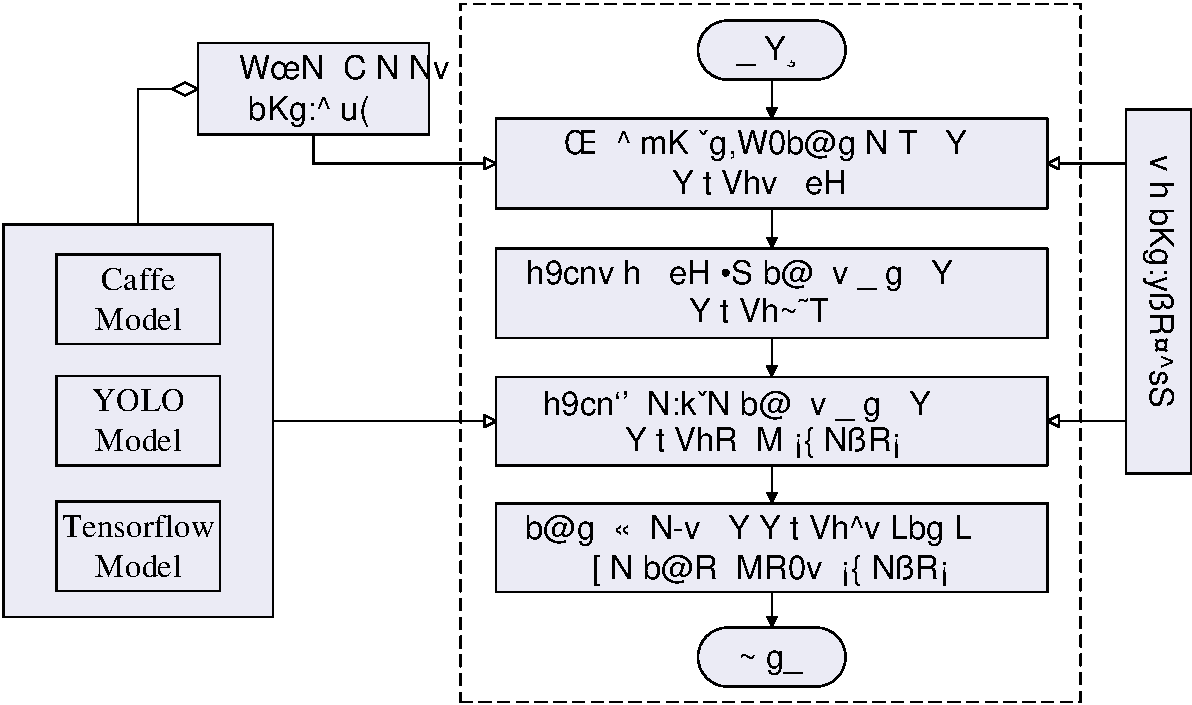
\includegraphics[height=0.4\textwidth]{figures/strategy_overview.pdf}
    \caption{基于异构计算的自适应计算任务分配策略概览}\label{figure:figure29}
\end{figure}

\subsection{高能效设备处理器组合的搜索}
\label{chapter:chapter4-3-1}

为了获得所期望的高能效设备处理器组合,首先需要了解目标手机移动平台上每一个可访问设备处理器的能效值。本文使用一种简单有效的方法来刻画目标平台上所有设备处理器的性能和能耗。简单来说,若目标平台上所有可访问的设备处理器数量为$n$,则在CNN运行时库的前$n$次运行中,每次都仅使用一个可访问的设备处理器执行完整的CNN推断。在每次执行完CNN推断后,推断过程在该设备上所需的执行时间、能耗、平均功耗以及EDP能效值会被记录下来。这一步会造成一些运行时开销,但是它仅仅发生在程序的前若干次运行中,因此这些开销会被程序的整个运行周期均摊。接下来,为了给设备选择操作做准备,每一个本地设备处理器的性能和功耗将会被正则化。最后,根据所期望的能效值不断剔除较低能效的设备处理器便可获得所需的高能效设备处理器组合。这里需要说明一点,对于同一应用,高能效设备处理器组合可被重复使用,因此整个搜索过程仅需执行一次。

\begin{algorithm}[htbp]
  \small
  \SetAlgoLined
    \begin{spacing}{0.8}
    \KwIn{(i) CNN模型结构参数和预训练的模型权重矩阵\;
          (ii) 能效阈值$EDP_{TH}$(默认值为1)。}
    \KwOut{所期望的高能效处理器组合$S_{HC}$以及组合中所有处理器的相对性能集$Perf$。}
    遍历目标平台上所有可访问的异构设备处理器(如GPUs,CPUs,NPUs等)并将它们放入设备集合$S_{HC}$中\;
    \For{$processor_i$ \textbf{in} $S_{HC}$} {
        使用处理器$processor_i$执行一次完整的CNN推断\;
        将本次推断的执行时间$t_i$, 能耗$e_i$以及平均功耗$p_i$分别存储到$T$,$E$和$P$三个数组中\;
        使用公式\ref{equation:equation1}计算本次推断的能效$EDP_i$并将其存储在$EDP$数组中\;
    }
    找出具有最小推断执行时间的处理器$processor_{min}$\;
    将$processor_{min}$的执行时间和平均功耗分别标记为$t_{min}$和$p_{ref}$\;
    \For{$(t_i$ \textbf{in} $T)$ \textbf{and} $(p_i$ \textbf{in} $P)$} {
    计算相对性能: $perf_{ri} = \frac{t_{min}}{t_i}$,将$perf_{ri}$添加到数组$Perf$中\;
    计算相对功耗:$p_{ri} = \frac{p_{i}}{p_{ref}}$,将$p_{ri}$添加到数组$P_r$中\;
    }
    \While{$edp_r < EDP_{TH}$}{
        计算相对执行时间:$t_r=\frac{1}{\sum_{perf \in Perf}perf}$\;
        计算相对总功耗:$p_{tr}={\sum_{pr \in P_r}pr}$\;
        计算相对能效EDP值:$edp_r=(p_{tr}*t_r)*t_r$\;
        \If {$edp_r \geq EDP_{TH}$}{
            找出具有最大EDP值的处理器,并记录其下标$i$\;
            从$S_{HC}$中移除$processor_i$\;
            从$Perf$中移除$perf_{ri}$\;
            从$P_r$中移除$p_{ri}$\;
        }
    }
    \textbf{return} $S_{HC}$和$Perf$\;
   \end{spacing}
  \caption{高能效设备处理器组合的搜索过程}
  \label{algo:algorithm8}
\end{algorithm}

算法\ref{algo:algorithm8}描述了在目标手机移动平台上进行高能效设备处理器组合搜索的核心过程。为了在手机本地端完成CNN前向推断过程,模型结构参数和权重矩阵的获取是必须的,这可以通过第\label{chapter:chapter3-2-1}章节提供的权重参数解析脚本实现。因为算法中使用了正则化处理,所以默认的能效阈值$EDP_{TH}$设置为1,这样可以使得在执行CNN推断时所选设备处理器组合的复合能效比任何一个单处理器的能效都要高。当然,用户也可以根据需要配置$EDP_{TH}$的值以得到不同的能效折中。

如算法\ref{algo:algorithm8}所示,CNN运行时库首先会遍历目标平台上所有可访问的异构设备处理器,如 GPUs,CPUs或NPUs等。然后,所有可获得的设备处理器被收集到一个容器中,这为接下来的搜索步骤做初始化工作(行1)。用户无需提前测量不同设备处理器的性能和功耗,因为本文提出的算法在CNN运行时库的前几次执行中会主动对每个可获得设备处理器的性能和功耗进行评估并进一步计算出它们的能效EDP值(行2-7)。

\subsection{计算任务的划分}
\label{chapter:chapter4-3-2}

\begin{algorithm}[htbp]
  \small
  \SetAlgoLined
    \begin{spacing}{0.9}
    \KwIn{所选设备处理器组合中所有处理器的相对性能集$Perf$。}
    \KwOut{所选组合中处理器所分配计算任务比例集$R$。}
    \For{$perf_{i}$ \textbf{in} $Perf$} {
        计算处理器$process_i$所分配任务比例:
        $$r=\frac{perf_{ri}}{\sum_{perf \in Perf}perf}$$
        将$r$添加到数组$R$中\;
    }
    \textbf{return} $R$\;
   \end{spacing}
  \caption{设备处理器组合中每一处理器所分配任务比例的计算过程}
  \label{algo:algorithm9}
\end{algorithm}